\chapter{Deriving template grammar from first principles}
    \section{Abstraction of composition}



        \subsection{Tree-substitution grammar}
    \section{Abstraction of repetition}
        What is a computational process that allow us from understanding 
        "catcat", "1414", "$\triangle\triangle$" as instantiations of same pattern $x \mapsto (x,x)$?

        Notice that these three examples are different in both their token types 
        and the length of the repeating unit.

        \subsection{Pattern language}
    \section{Abstraction of composition with repeat}
        \subsection{Repetition combinators}

        Let $f : A \to B, g: X \to Y$ their tensor product is defined as
        \begin{align*}
            f \otimes g : A \times X  &\to B \times Y\\
            (f \otimes g)(a,x) &= (b,y)
        \end{align*}
        It is further required that this tensor product is associative, i.e. $(f \circ g) \circ h \simeq f \circ (g \circ h)$.

        $$
        (g, (f_1,...,f_n)) \mapsto g \circ (m_g(f_1,...,f_n))
        $$
        where $m_g$ is a function that duplicates its $n$ inputs into $k$ outputs where $n\leq k$.  
        $$
        m_g (f_1,...,f_n)= g\circ \bigotimes_{i=1}^k f'_i  \quad \text{where} \quad 
        f'_i \in \{g,f_1,...,f_n\}
        $$
        The set of all such functions can be defined constructively
        

        \subsection{Introducing template grammar}
            \begin{align}
                \mathbb S &:= \_\_ \ | \ \star \ |\  \mathbb N^+ \\
                \mathbb M &:= \mathbb S ^ *\\
                \mathcal T &:= E \ |\  (\mathbb N, \mathcal T, \mathcal T) \ |\  (\mathcal T, \mathbb M, \mathcal T^*)
            \end{align}

            
            

        \subsection{Template grammar as a probabilistic program}
        
\pgfmathsetmacro {\vizWidth}{0.24}
\chapter{Parsing of Template grammar}
    \section{Parsing as weighted deduction} 
    \section{A polynomial time semi-ring parsing algorithm}
    \subsection{Notations}
        Like a production rule, a template $\alpha \in \mathcal T$ may expand a non-terminal $X \in NT$ into 
        a list of symbols. The resulted $n$ non-terminals divides the terminals into $n+1$ chunks.
        We call these chunks as the \emph{evidence} of $\alpha$ on $X$. 
        We denote this ternary relations among 
        a head non-terminal $X$, a template $X$, and an evidence $e$ as $X \xrightarrow{\alpha} e$
        
        The goal of parsing template grammar is to understand how 
        a list of list of terminals, as the evidence for some template on the start symbol $S$. 
        \subsubsection{Item form:} 
            Each item is a triple $(NT, \mathcal{T},{T^*}^*)$ denoted as 
            \begin{equation} {X \xrightarrow{\alpha} e}
            \end{equation}
            which corresponds to the proposition "the evidence resulted from 
            template $\alpha$ on the non-terminal $X$ is $e$"
        
        

         
        \subsubsection{Inference rules}

        % \setlength{\tabcolsep}{15pt}
        % \renewcommand{\arraystretch}{1}
        \begin{tabular}{l c c}

            \midrule\\
            \textbf{Zero-hole}\\
            
            $\textsc{Complete}^{\langle \_ \rangle}_0$  &
            \begin{minipage}{\vizWidth\textwidth}
                \medskip
                {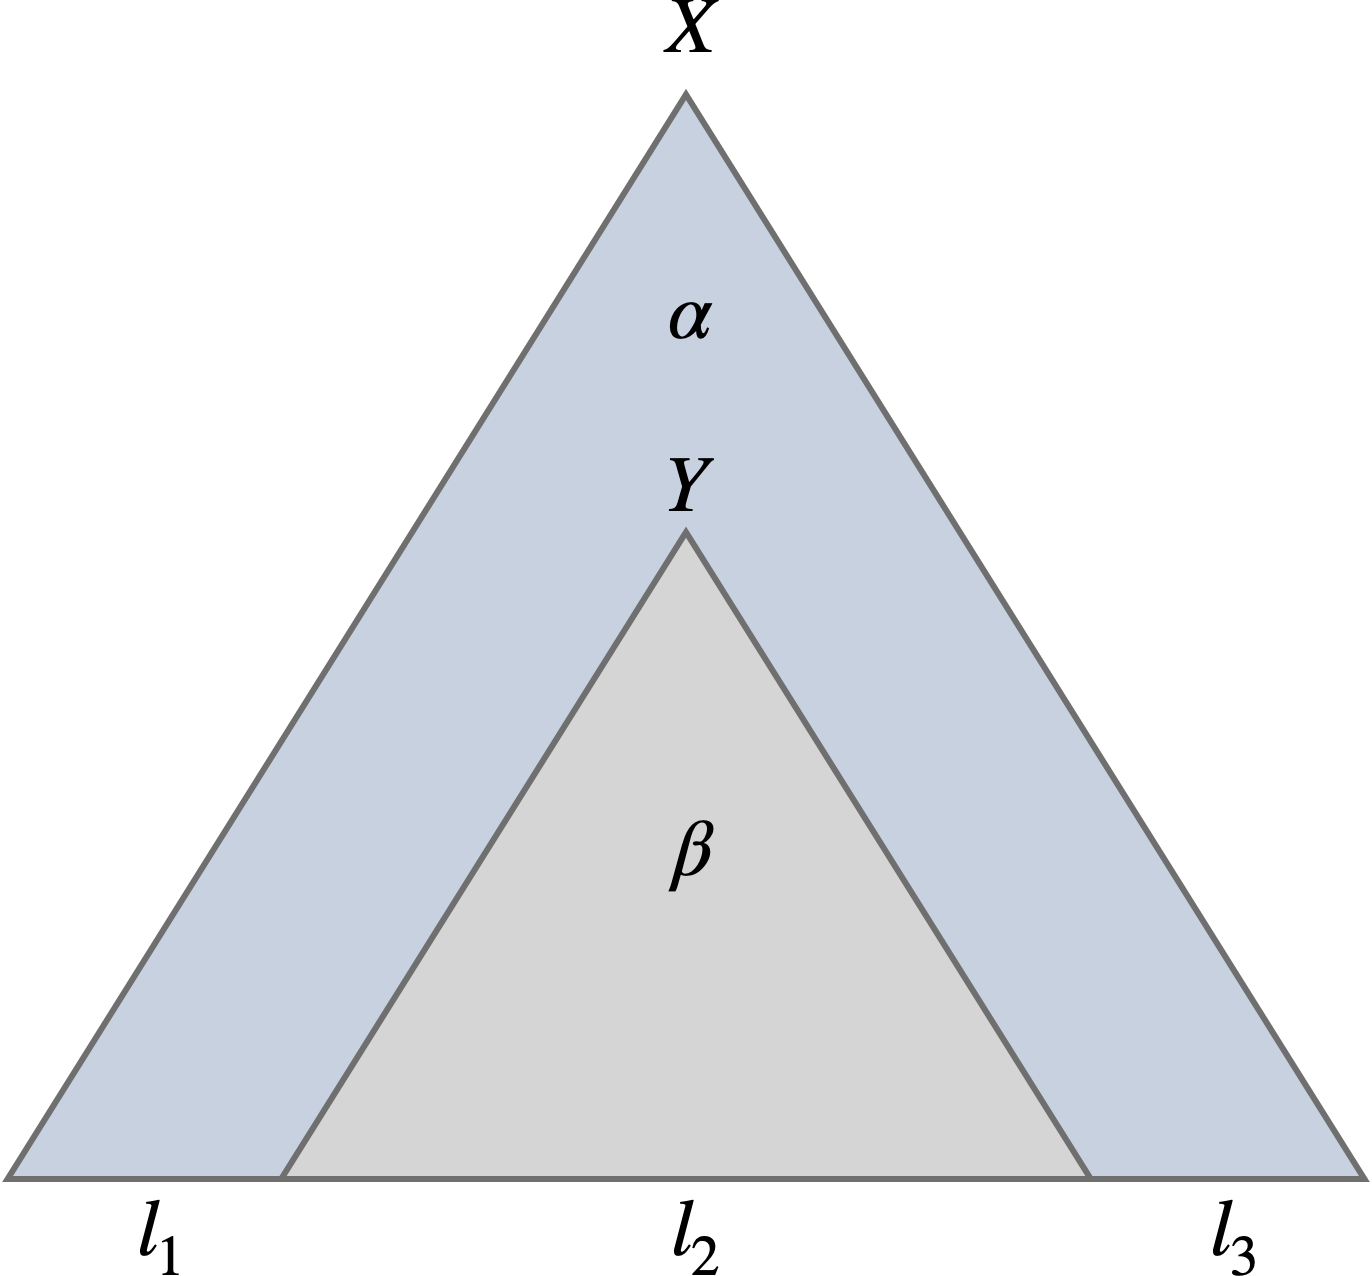
\includegraphics[width=\linewidth]{images/parsing/complete[New][0].png}}
            \end{minipage} &
            \AxiomC{$X \xrightarrow{\alpha} [l_1,l_3]$}
            \AxiomC{$Y \xrightarrow{\beta} [l_2]$}
            \RightLabel{$\substack {l_2 \neq [\ ] \\ X \overset{\alpha}{\leadsto}  [Y]}$}
            \BinaryInfC{$X \xrightarrow {(\alpha,\langle \_\rangle, [\beta])} {[l_1+l_2+l_3]}$}
            \DisplayProof\\
            
           
            $\textsc{Complete}^{\langle \_ \  \_ \rangle}_{0,0}$ &
            \begin{minipage}{\vizWidth\textwidth}
                \medskip
                {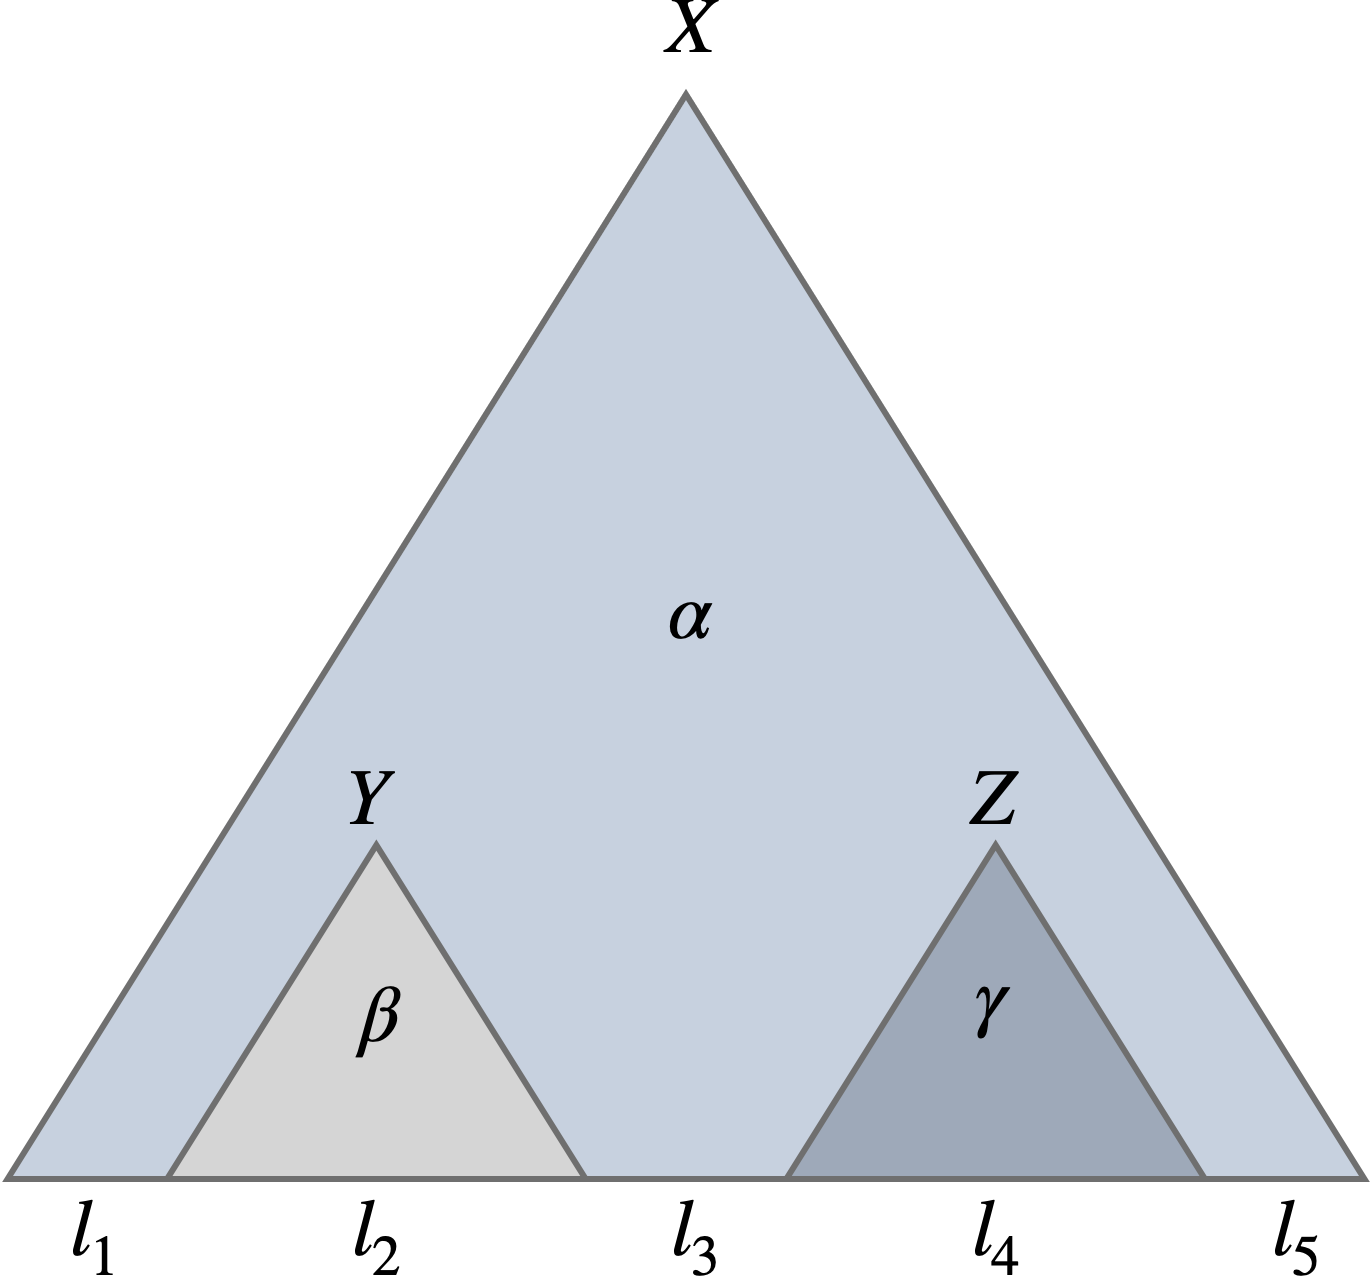
\includegraphics[width=\linewidth]{images/parsing/complete[New,New][0,0].png}}
            \end{minipage} &
            \AxiomC{$X \xrightarrow{\alpha} [l_1,l_3,l_5] $}
            \AxiomC{$Y \xrightarrow{\beta} [l_4]$}
            \AxiomC{$Z \xrightarrow{\gamma} [l_4]$}
            \RightLabel{$\substack{l_2,l_4 \neq [\ ] \\ X \overset{\alpha}{\leadsto} [Y,Z]}$}
            \TrinaryInfC{$X \xrightarrow {(\alpha,\langle \_ \ \_ \rangle, [\beta, \gamma])} {[l_1+l_2+l_3+l_4+l_5]}$}
            \DisplayProof\\
            
            
            $\textsc{Complete}^{\langle \_ \  1 \rangle}_{0,0}$ &
            \begin{minipage}{\vizWidth\textwidth}
                \medskip
                {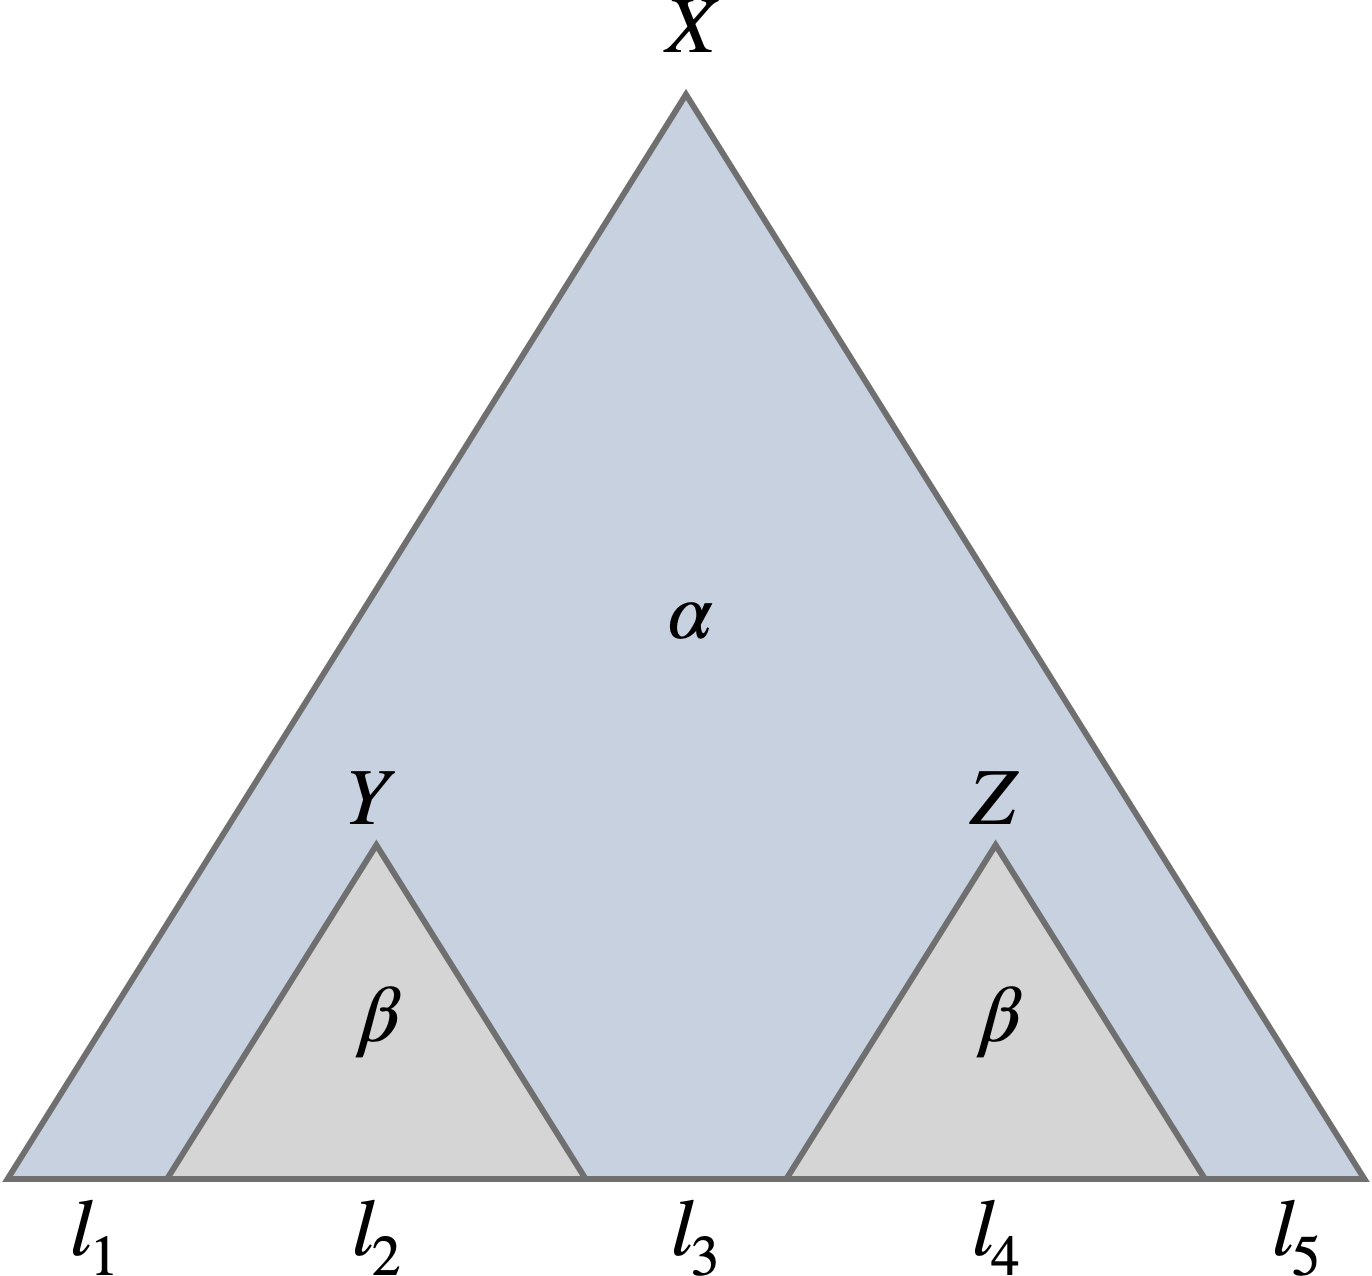
\includegraphics[width=\linewidth]{images/parsing/complete[New,1][0,0].png}}
            \end{minipage} &
            \AxiomC{$X \xrightarrow{\alpha} [l_1,l_3,l_5] $}
            \AxiomC{$Y \xrightarrow{\beta} [l_4]$}
            \AxiomC{$Z \xrightarrow{\beta} [l_4]$}
            \RightLabel{$\substack{l_2,l_4 \neq [\ ] \\ X \overset{\alpha}{\leadsto} [Y,Z]}$}
            \TrinaryInfC{$X \xrightarrow {(\alpha,\langle \_ 1 \rangle, [\beta])} {[l_1+l_2+l_3+l_4+l_5]}$}
            \DisplayProof
        \end{tabular}
        
        
        \begin{tabular}{l c l}
            \midrule\\
            \textbf{One-hole}\\

            $\textsc{Complete}^{\langle \star \rangle}_1$ &
            \begin{minipage}{\vizWidth\textwidth}
                \smallskip
                {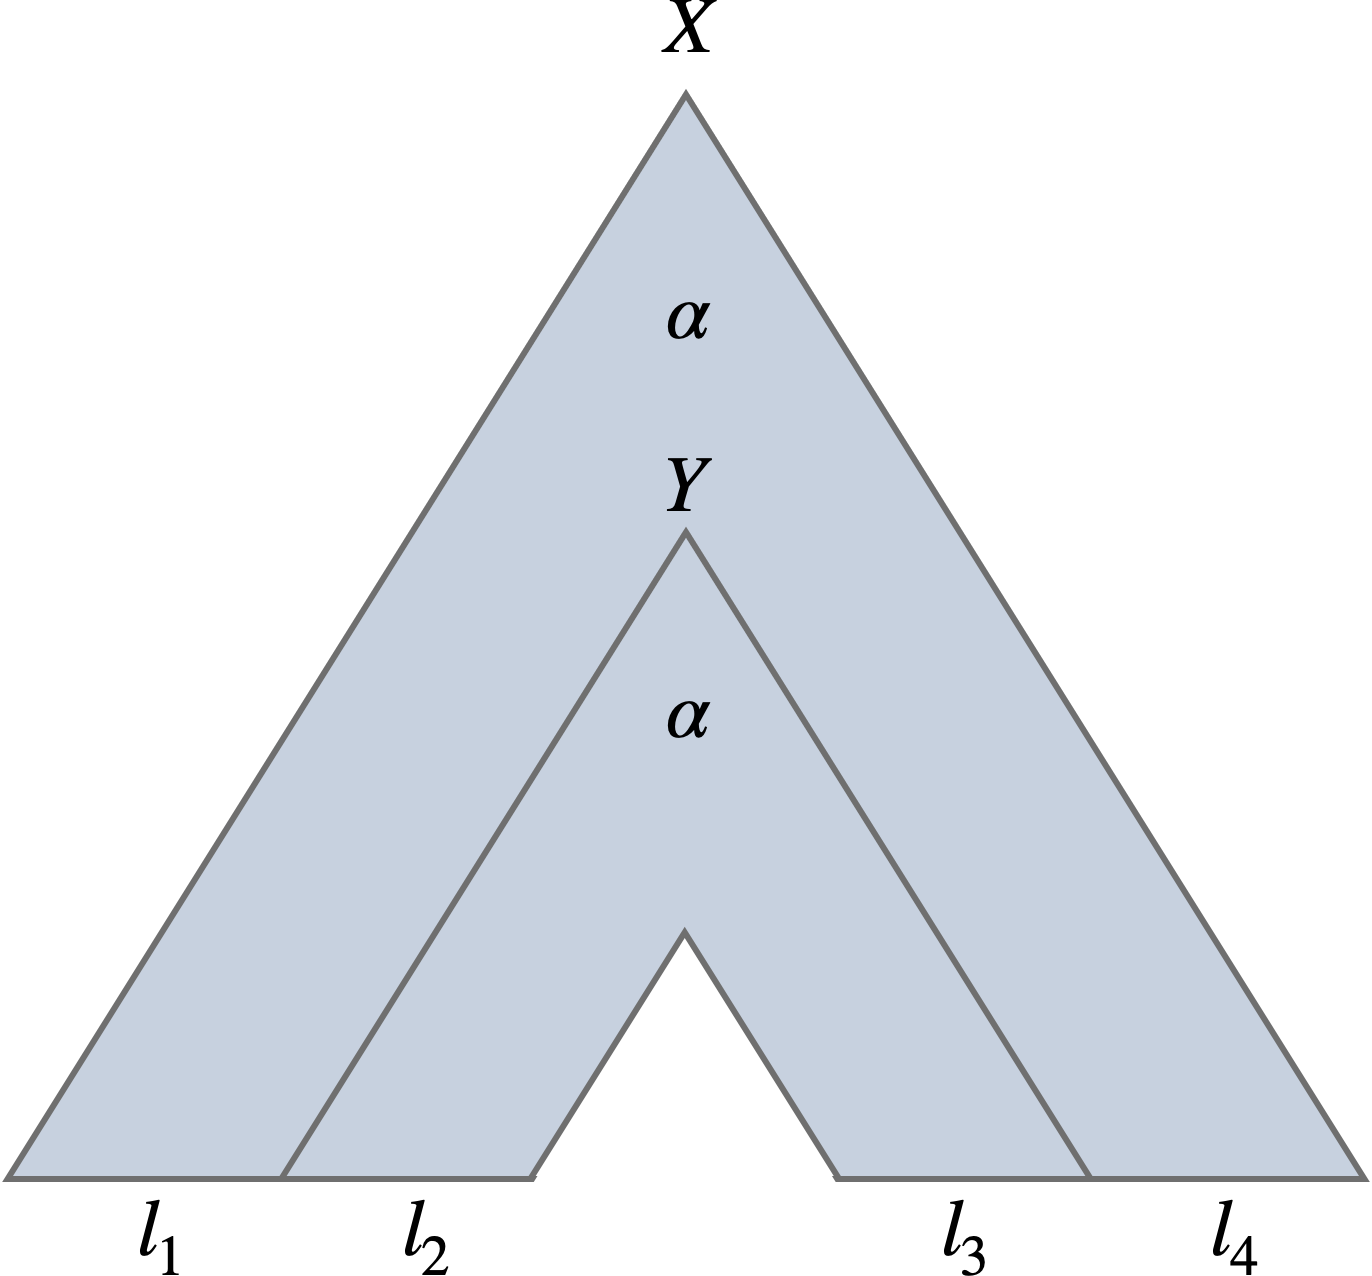
\includegraphics[width=\linewidth]{images/parsing/complete[Star][1].png}}
            \end{minipage} &
            \AxiomC{$X \xrightarrow{\alpha} [l_1,l_4] $}
            \AxiomC{$Y \xrightarrow{\alpha} [l_2,l_3]$}
            \RightLabel{$\substack {X \overset{\alpha}{\leadsto} [Y]}$}
            \BinaryInfC{$X \xrightarrow {(\alpha,\langle \star \rangle, [\ ])} {[l_1+l_2,l_3+l_4]}$}
            \DisplayProof\\
        
            $\textsc{Complete}^{\langle \_ \rangle}_1$ &
            \begin{minipage}{\vizWidth\textwidth}
                \smallskip
                {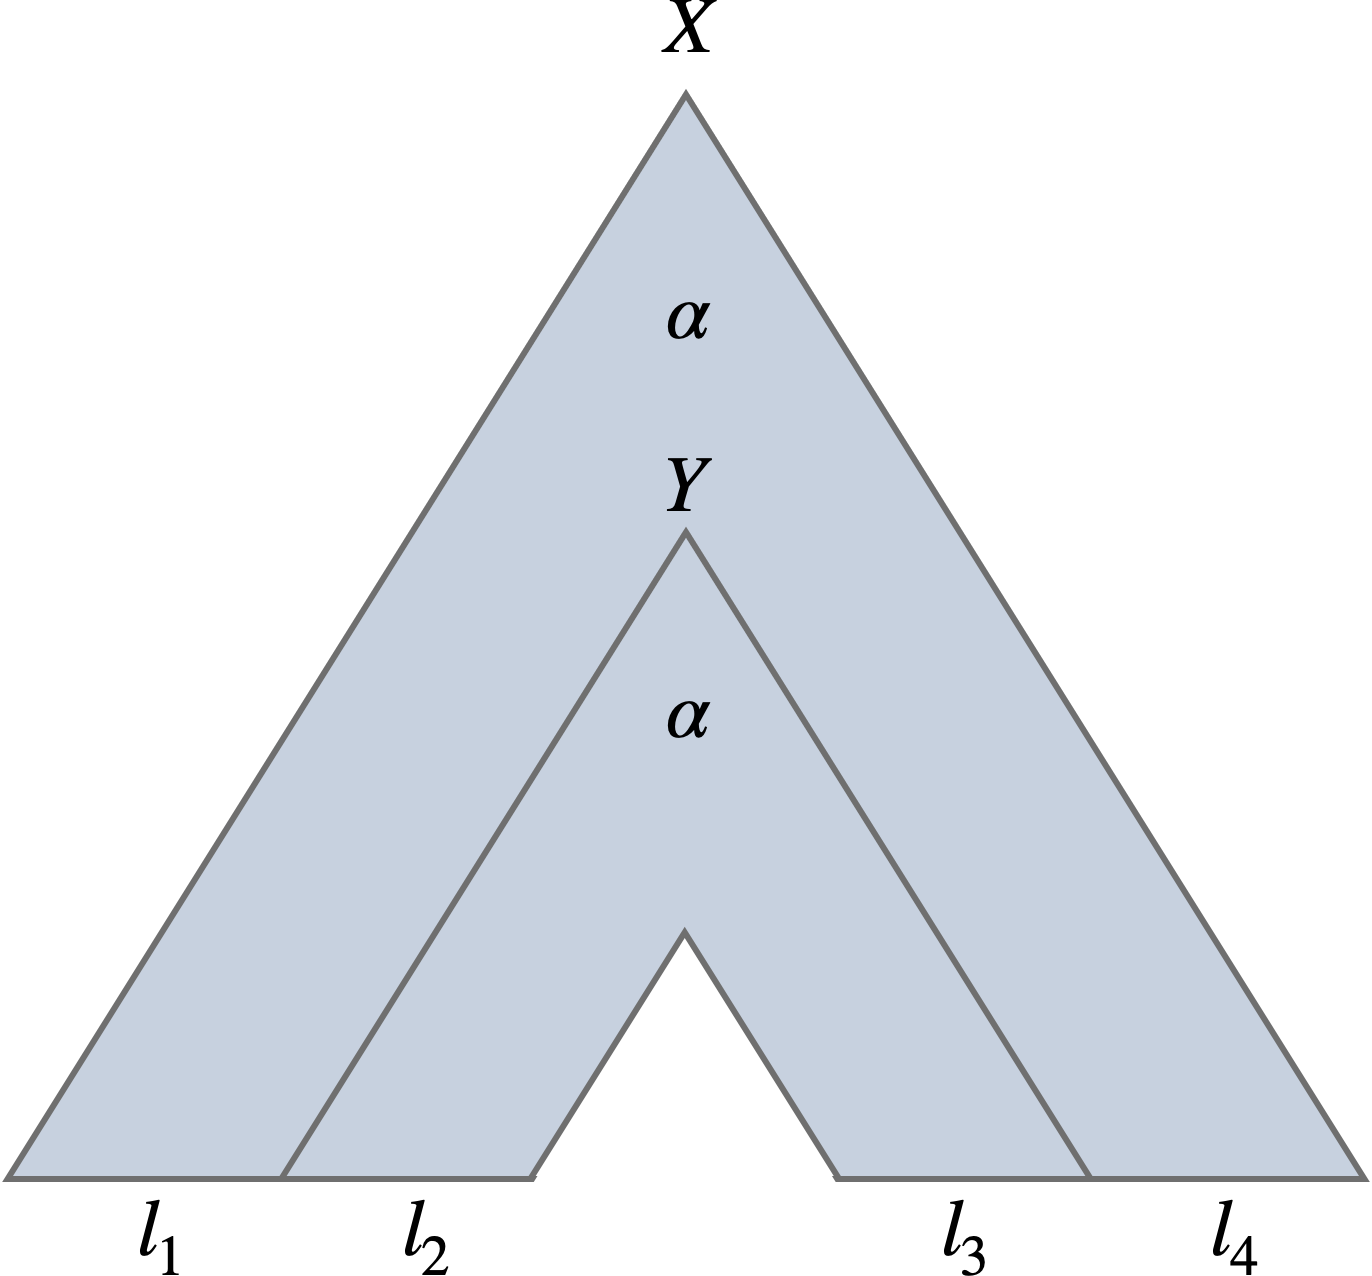
\includegraphics[width=\linewidth]{images/parsing/complete[Star][1].png}}
            \end{minipage} &
            \AxiomC{$X \xrightarrow{\alpha} [l_1,l_4]$}
            \AxiomC{$Y \xrightarrow{\beta} [l_2,l_3]$}
            \RightLabel{$\substack {X \overset{\alpha}{\leadsto} [Y]}$}
            \BinaryInfC{$X \xrightarrow {(\alpha,\langle \_\rangle, [\beta])} {[l_1+l_2,l_3+l_4]}$}
            \DisplayProof
        \end{tabular}
        
       
    

        \subsection{Proof of correctness}
    \section{Approximate parsing for Template grammar}
        \subsection{Tree compression}
        \subsection{A-star parsing}